\chapter{Data Wrangling and Feature Construction}
\label{ch:wrangling}
\chapterguide
  {You should understand observations, variables, data types, and data-quality checks.}
  {select and filter records, sort data, compute grouped summaries, and create features that preserve clear meaning.}

\section{Wrangling changes representation, not the question}
Data wrangling prepares the evidence needed for analysis. Common operations are selecting variables, filtering observations, ordering records, grouping categories, aggregating summaries, joining tables, and constructing derived features.

\begin{utpfig}[Wrangling pipeline]{Each operation should be explainable as a transformation from one table to another.}{fig:wrangling-pipeline}
\begin{tikzpicture}[x=\linewidth,y=1cm,
  stage/.style={draw=UTPBlue!65,fill=UTPPaleBlue,rounded corners=1.8mm,
    line width=0.7pt,text width=0.14\linewidth,
    minimum width=0.18\linewidth,minimum height=1.70cm,
    inner xsep=2.5mm,inner ysep=2.5mm,align=center,
    font=\scriptsize\color{UTPNavy}},
  endpoint/.style={stage,draw=UTPTeal!80,fill=UTPPaleTeal},
  flow/.style={-{Stealth[length=2mm,width=1.5mm]},
    line width=0.9pt,draw=UTPTeal}]
\node[endpoint] (raw) at (0.10,0)
  {\textcolor{UTPTeal}{\textbf{01  INPUT}}\\[5pt]
   \textbf{Raw table}\\[3pt]
   Original records\\and variables};
\node[stage] (sel) at (0.30,0)
  {\textcolor{UTPBlue}{\textbf{02  SCOPE}}\\[5pt]
   \textbf{Select and filter}\\[3pt]
   Relevant rows\\and columns};
\node[stage] (feat) at (0.50,0)
  {\textcolor{UTPBlue}{\textbf{03  DERIVE}}\\[5pt]
   \textbf{Create features}\\[3pt]
   Interpretable\\derived variables};
\node[stage] (grp) at (0.70,0)
  {\textcolor{UTPBlue}{\textbf{04  SUMMARISE}}\\[5pt]
   \textbf{Aggregate}\\[3pt]
   Summaries at\\the required grain};
\node[endpoint] (ana) at (0.90,0)
  {\textcolor{UTPTeal}{\textbf{05  OUTPUT}}\\[5pt]
   \textbf{Analysis table}\\[3pt]
   Evidence for\\the question};
\draw[flow] (raw.east) -- (sel.west);
\draw[flow] (sel.east) -- (feat.west);
\draw[flow] (feat.east) -- (grp.west);
\draw[flow] (grp.east) -- (ana.west);
\end{tikzpicture}
\end{utpfig}


\section{Think in verbs: each step should have one purpose}
A readable wrangling pipeline is a sequence of simple verbs: \emph{select}, \emph{filter}, \emph{mutate}, \emph{group}, \emph{summarise}, \emph{join}, and \emph{reshape}. Keeping transformations small makes intermediate row counts and assumptions easier to audit.

\begin{utpfig}[Table transformations as contracts]{Each transformation should preserve a clear contract: what one row represents, which variables are retained, and which new values were derived.}{fig:wrangle-contract}
\begin{tikzpicture}[node distance=0.14cm,
  stage/.style={draw=UTPBlue!65,fill=UTPPaleBlue,rounded corners=1.8mm,
    line width=0.7pt,text width=0.70\linewidth,
    minimum width=0.76\linewidth,minimum height=0.84cm,
    inner xsep=5mm,inner ysep=1.3mm,align=left,
    font=\scriptsize\color{UTPNavy}},
  endpoint/.style={stage,draw=UTPTeal!80,fill=UTPPaleTeal},
  flow/.style={-{Stealth[length=1.8mm,width=1.4mm]},
    line width=0.9pt,draw=UTPTeal},
  stagejoin/.style={line width=0.75pt,draw=UTPTeal}]
\node[endpoint] (a)
  {\textcolor{UTPTeal}{\textbf{01  INPUT CONTRACT}}\\[3pt]
   One row = one wine sample; 15 variables};
\node[stage,below=of a] (b)
  {\textcolor{UTPBlue}{\textbf{02  SELECT}}\\[3pt]
   Keep cultivar, alcohol, colour intensity, and proline};
\node[stage,below=of b] (c)
  {\textcolor{UTPBlue}{\textbf{03  FILTER}}\\[3pt]
   Retain records meeting a stated inclusion rule};
\node[stage,below=of c] (d)
  {\textcolor{UTPBlue}{\textbf{04  CREATE FEATURES}}\\[3pt]
   Add interpretable derived columns};
\node[endpoint,below=of d] (e)
  {\textcolor{UTPTeal}{\textbf{05  OUTPUT CONTRACT}}\\[3pt]
   One row still = one wine sample; analysis-ready variables};
\coordinate (r1) at ([xshift=-7mm]a.west);
\coordinate (r2) at ([xshift=-7mm]b.west);
\coordinate (r3) at ([xshift=-7mm]c.west);
\coordinate (r4) at ([xshift=-7mm]d.west);
\coordinate (r5) at ([xshift=-7mm]e.west);
\draw[flow] ([yshift=3mm]r1) -- ([yshift=-3mm]r5);
\foreach \rail/\card in {r1/a,r2/b,r3/c,r4/d,r5/e}{
  \draw[stagejoin] (\rail) -- (\card.west);
  \fill[UTPTeal] (\rail) circle (1.15pt);
}
\end{tikzpicture}
\end{utpfig}

\section{Select only what the question needs}
If the question concerns alcohol, colour intensity, and cultivar, carrying every available variable into every step increases cognitive load and opportunities for mistakes.

\begin{lstlisting}[style=utpr]
analysis <- wine[, c("cultivar", "alcohol",
                     "color_intensity", "proline")]
\end{lstlisting}

\section{Filter records with explicit conditions}
Filtering defines the population being analysed. That means every filter should be stated in the report.

\begin{lstlisting}[style=utpr]
high_alcohol <- wine[wine$alcohol >= 13.5, ]
\end{lstlisting}

\begin{pitfall}
Filtering after looking at the outcome can quietly turn exploration into cherry-picking. Define inclusion rules from the analytical question or domain constraints, and disclose post-hoc filters.
\end{pitfall}


\section{Aggregation changes the unit of observation}
When rows are grouped and summarised, the output table no longer represents individual observations. One row may now represent a cultivar, region, month, or customer. This is a fundamental change in the analytical unit and should be made explicit.

\begin{utpfig}[Grouped means with uncertainty]{The cultivar means differ, while the dashed line shows the overall mean. Error bars are approximate 95\% intervals for each group mean and remind us that summaries are estimates.}{fig:wrangle-group-summary}
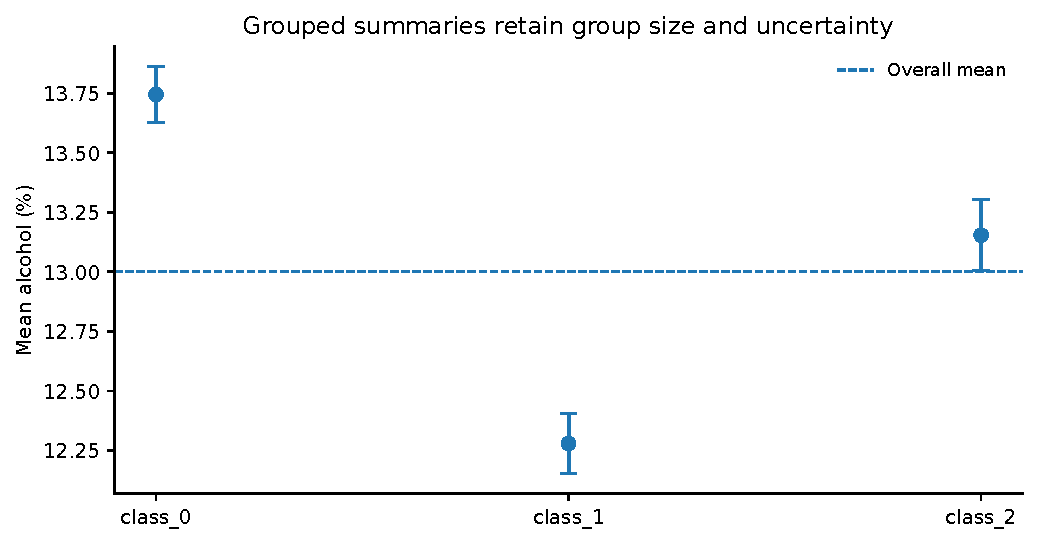
\includegraphics[width=0.80\linewidth]{figures/wrangling_group_summary.pdf}
\end{utpfig}


\begin{utpfig}[A transformation changes scale and shape]{The log transformation compresses large values more strongly than small values. It can make skewed data easier to visualise or model, but it also changes coefficient interpretation.}{fig:wrangle-transform}
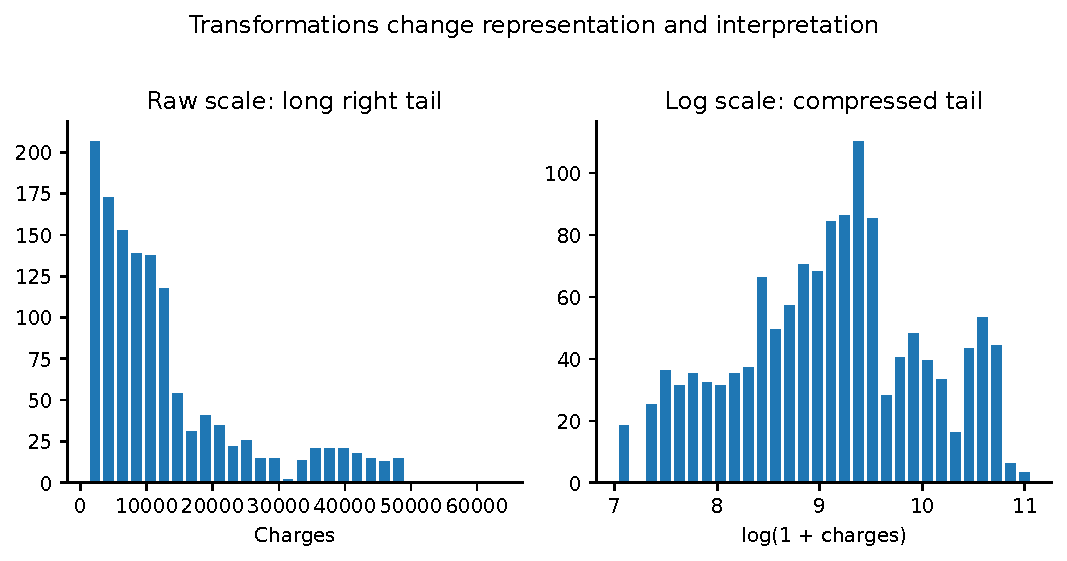
\includegraphics[width=0.82\linewidth]{figures/wrangling_transform.pdf}
\end{utpfig}

\begin{keyidea}
Always ask whether a grouped result is weighted correctly for the question. Averaging three group means is not generally the same as the overall mean when group sizes differ.
\end{keyidea}

\section{Grouped summaries reveal structured differences}
Overall averages can hide subgroup structure. The \cmd{aggregate()} function makes the comparison explicit:
\begin{lstlisting}[style=utpr]
aggregate(alcohol ~ cultivar, data = wine, FUN = mean)
\end{lstlisting}
A group summary should usually include both a center and a measure of spread or sample size.


\section{Reshaping: wide and long representations}
The same information can be represented in different table shapes. \term{Wide} data often place repeated measures in separate columns, while \term{long} data place the measurement name and value in rows. Long form is often convenient for grouped plotting and repeated-measures analysis; wide form can be convenient for modelling matrices.

\begin{utpfig}[Wide and long are representations of the same information]{Reshaping should change layout, not invent or discard measurements. The key columns must be sufficient to reconstruct the original representation.}{fig:wide-long}
\begin{tikzpicture}[x=\linewidth,y=1cm,
  tablecard/.style={draw=UTPBlue!65,fill=UTPPaleBlue,rounded corners=1.8mm,
    line width=0.7pt,text width=0.36\linewidth,
    minimum width=0.42\linewidth,minimum height=4.05cm,
    inner sep=3mm,align=center,font=\scriptsize\color{UTPNavy}},
  reshapebadge/.style={draw=UTPTeal!80,fill=UTPPaleTeal,
    rounded corners=4mm,line width=0.75pt,text width=0.075\linewidth,
    minimum height=0.78cm,inner xsep=2mm,inner ysep=1.5mm,
    align=center,font=\scriptsize\bfseries\color{UTPTeal}},
  reshape/.style={-{Stealth[length=2mm,width=1.5mm]},
    line width=0.85pt,draw=UTPTeal}]
\node[tablecard] (wide) at (0.22,0) {%
  \begin{minipage}[t][3.35cm][t]{\linewidth}
  \setlength{\parskip}{0pt}
  \centering
  \textcolor{UTPBlue}{\textbf{01  WIDE FORMAT}}\\[3pt]
  \textbf{One row per ID}\\[1pt]
  Repeated measures occupy columns\par\vspace{4pt}
  \fontsize{7.4}{8.8}\selectfont
  \renewcommand{\arraystretch}{1.02}
  \setlength{\tabcolsep}{5pt}
  \setlength{\extrarowheight}{0pt}
  \arrayrulecolor{UTPBlue!45}
  \begin{tabular}{@{}crr@{}}
  \rowcolor{UTPBlue!85}
  \textcolor{white}{\textbf{ID}} &
  \textcolor{white}{\textbf{Morning}} &
  \textcolor{white}{\textbf{Evening}} \\
  \rowcolor{white}
  01 & 21.4 & 26.1 \\
  \rowcolor{UTPBlue!5}
  02 & 20.9 & 25.6 \\
  \bottomrule
  \end{tabular}
  \end{minipage}};
\node[tablecard,draw=UTPTeal!80,fill=UTPPaleTeal] (long) at (0.78,0) {%
  \begin{minipage}[t][3.35cm][t]{\linewidth}
  \setlength{\parskip}{0pt}
  \centering
  \textcolor{UTPTeal}{\textbf{02  LONG FORMAT}}\\[3pt]
  \textbf{One row per ID and time}\\[1pt]
  Repeated measures occupy rows\par\vspace{4pt}
  \fontsize{7.4}{8.8}\selectfont
  \renewcommand{\arraystretch}{1.02}
  \setlength{\tabcolsep}{5pt}
  \setlength{\extrarowheight}{0pt}
  \arrayrulecolor{UTPTeal!45}
  \begin{tabular}{@{}clr@{}}
  \rowcolor{UTPTeal!85}
  \textcolor{white}{\textbf{ID}} &
  \textcolor{white}{\textbf{Time}} &
  \textcolor{white}{\textbf{Value}} \\
  \rowcolor{white}
  01 & morning & 21.4 \\
  \rowcolor{UTPTeal!5}
  01 & evening & 26.1 \\
  \rowcolor{white}
  02 & morning & 20.9 \\
  \rowcolor{UTPTeal!5}
  02 & evening & 25.6 \\
  \bottomrule
  \end{tabular}
  \end{minipage}};
\node[reshapebadge] (change) at (0.50,0)
  {RESHAPE};
\draw[reshape] (wide.east) -- (change.west);
\draw[reshape] (change.east) -- (long.west);
\node[font=\scriptsize\color{UTPMuted},align=center] at (0.50,-2.30)
  {same measurements \textbullet\ different layout};
\end{tikzpicture}
\end{utpfig}

\section{Feature engineering should add meaning}
A \term{feature} is an input variable used in analysis or modelling. New features can simplify relationships, encode domain knowledge, or make scales easier to compare.

\begin{utptable}
\begin{tabularx}{\linewidth}{@{}>{\bfseries\leavevmode\color{UTPNavy}}m{3.1cm}D{4.4cm}Y@{}}
\toprule
\rowcolor{UTPPaleBlue!92}
\utpth{Feature operation} & \utpth{Example} & \utpth{Reason} \\
\midrule
Binning & alcohol to lower/middle/higher & communicate broad ranges \\
Transformation & \(\log(1+x)\) & compress strongly right-skewed values \\
Ratio & cost per unit & represent relative rather than absolute size \\
Interaction & age \(\times\) treatment & allow one effect to vary with another \\
Indicator & missing = yes/no & preserve missingness as information \\
\bottomrule
\end{tabularx}
\end{utptable}

\begin{keyidea}
A good engineered feature has a sentence-level interpretation. If you cannot explain what the feature means without referring to the code that produced it, it is hard to defend analytically.
\end{keyidea}


\section{Join cardinality should be known before the join}
A join combines rows according to key matches. The expected relationship between keys is called \term{cardinality}. One-to-one joins should preserve row count; one-to-many joins deliberately repeat the ``one'' side; many-to-many joins can create a Cartesian multiplication and are frequently accidental.

\begin{utpfig}[Join cardinality]{Knowing the expected key relationship lets row-count changes become a diagnostic rather than a surprise.}{fig:join-cardinality}
\begin{tikzpicture}[x=\linewidth,y=1cm,
  relationship/.style={draw=UTPBlue!65,fill=UTPPaleBlue,
    rounded corners=1.8mm,line width=0.7pt,text width=0.235\linewidth,
    minimum width=0.29\linewidth,minimum height=2.70cm,
    inner xsep=4mm,inner ysep=3mm,
    align=center,font=\scriptsize\color{UTPNavy}}]
\node[relationship] (oneone) at (0.17,0)
  {\textcolor{UTPBlue}{\textbf{01  ONE-TO-ONE}}\\[5pt]
   {\fontsize{13}{15}\selectfont\bfseries 1 : 1}\\[6pt]
   One profile per ID\\One outcome per ID\\[6pt]
   \textcolor{UTPMuted}{\textbf{ROW COUNT}}\\[-1pt]
   Usually preserved};
\node[relationship,draw=UTPTeal!80,fill=UTPPaleTeal] (onemany) at (0.50,0)
  {\textcolor{UTPTeal}{\textbf{02  ONE-TO-MANY}}\\[5pt]
   {\fontsize{13}{15}\selectfont\bfseries 1 : many}\\[6pt]
   One customer\\Many transactions\\[6pt]
   \textcolor{UTPMuted}{\textbf{ROW COUNT}}\\[-1pt]
   Expected expansion};
\node[relationship,draw=UTPRed!80,fill=UTPPaleRed] (manymany) at (0.83,0)
  {\textcolor{UTPRed!85!black}{\textbf{03  MANY-TO-MANY}}\\[5pt]
   {\fontsize{13}{15}\selectfont\bfseries many : many}\\[6pt]
   Repeated keys\\on both sides\\[6pt]
   \textcolor{UTPRed!85!black}{\textbf{ROW COUNT}}\\[-1pt]
   Can multiply unexpectedly};
\end{tikzpicture}
\end{utpfig}

\section{Joining tables introduces a new failure mode}
When combining tables, the join key should be unique at the expected level. A many-to-many join can multiply rows and corrupt counts.

\begin{workedexample}
Before joining customer and transaction tables, verify whether customer ID is unique in the customer table and repeated in the transaction table. That expected one-to-many relationship is part of the data model, not an implementation detail.
\end{workedexample}

\begin{quickcheck}
\begin{enumerate}
  \item Why can an overall mean be misleading when groups differ strongly?
  \item What should be stated whenever rows are filtered out?
  \item Give one reason to log-transform a feature.
  \item What join problem can cause row counts to increase unexpectedly?
\end{enumerate}
\end{quickcheck}

\section{Worked case: from 17,379 hourly rows to an interpretable demand profile}

The hourly Bike Sharing file demonstrates why wrangling is analytical work rather than clerical preparation. One row represents one observed hour. The goal is not to make the table smaller for its own sake, but to create a representation matched to a question such as ``How does the daily demand pattern differ between working and non-working days?''

\begin{utpfig}[Aggregation exposes a behavioural pattern]{A grouped hourly summary reveals commuting peaks on working days and a broader daytime pattern on non-working days. The transformation changes the grain from individual observed hours to mean demand for each hour--day-type combination.}{fig:wrangle-bike-hours}
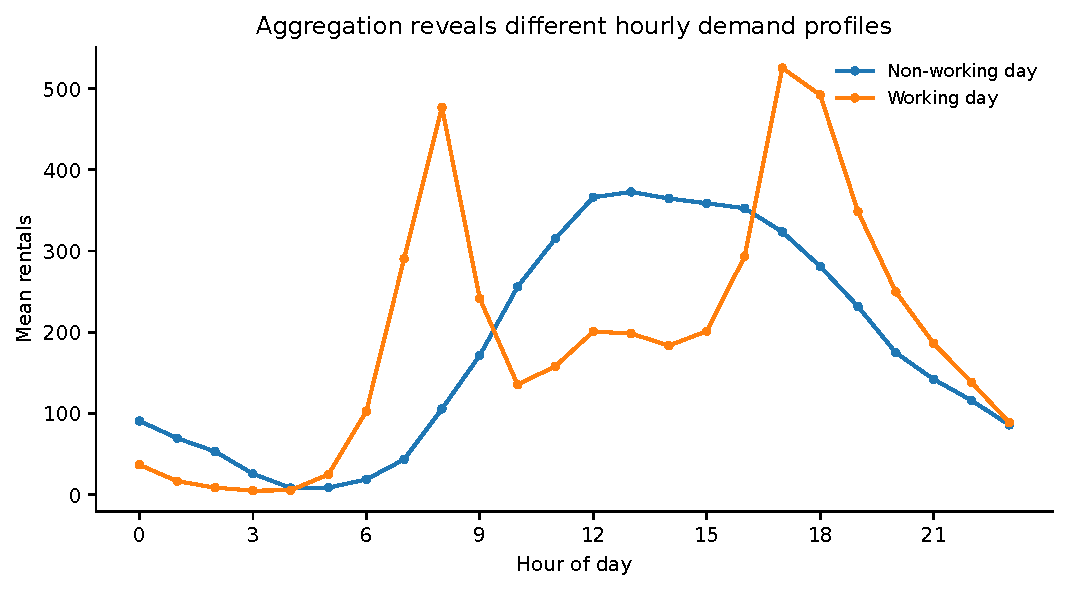
\includegraphics[width=0.86\linewidth]{figures/wrangling_bike_hourly_profiles.pdf}
\end{utpfig}

A useful feature engineering detail is that clock hour is cyclical. In ordinary numeric distance, hours 23 and 0 appear 23 units apart even though they are adjacent on the clock. A common encoding maps hour to the unit circle:
\[
  h_{\sin}=\sin(2\pi h/24), \qquad h_{\cos}=\cos(2\pi h/24).
\]
This representation preserves neighbourhood around midnight and gives models two smooth numeric variables instead of an arbitrary linear scale.

\begin{keyidea}
Every aggregation changes the unit of analysis. Before and after a \cmd{group}/\cmd{summarise} operation, state what one row represents. Many subtle data errors are actually grain errors.
\end{keyidea}

\labsection{3}{Reshape time-aware data and engineer defensible features}{sec:lab03}

\begin{labproject}{Wrangling and feature engineering: build an analysis-ready table}
\textbf{Coverage.} Chapter~\ref{ch:wrangling}.\\
\textbf{Goal.} You should be able to preserve observational grain, construct derived variables, aggregate intentionally, validate engineered features, and explain what information is lost when data are summarised.\\
\textbf{Dataset.} \texttt{bike\_sharing\_dataset\_hour.csv}.\\
\textbf{Scenario.} Hourly bike records are too granular for a manager who wants to understand commuting demand. Your task is to transform the source table into a compact, traceable analytical dataset without losing the meaning of the original measurements.

\textbf{Core workflow.}
\begin{enumerate}
  \item \textbf{State the grain.} Confirm that one row represents one observed hour on one date. Verify the date and hour ranges before any transformation.
  \item \textbf{Preserve raw variables.} Create readable day-type and hour labels as new fields rather than replacing coded source columns.
  \item \textbf{Engineer an operational feature.} Define peak-period categories with explicit hour boundaries. Explain why the chosen boundaries are analytical assumptions rather than facts stored in the data.
  \item \textbf{Represent cyclical time.} Create sine/cosine encodings for hour-of-day so that 23:00 is close to 00:00 in feature space. Verify the unit-circle identity numerically.
  \item \textbf{Aggregate for a question.} Produce mean rental profiles by hour and working-day status. State how the observational unit changes after aggregation.
  \item \textbf{Separate demand components.} Summarise \texttt{casual} and \texttt{registered} rentals by peak period and day type. Identify where the two user groups show materially different patterns.
  \item \textbf{Validate the transformation.} Check that group counts sum to the source row count, engineered categories contain no unexpected missing values, and total rentals remain consistent with their components.
\end{enumerate}

\begin{tryit}
\textbf{Extension.} Change one peak-period boundary and quantify how much the resulting group summaries change. Use the result to explain why feature engineering should be treated as a modelling decision that may require sensitivity analysis.
\end{tryit}

\tcbbreak
\lstinputlisting[style=utpr]{all_experiments/lab03_wrangling.R}
\begin{verification}
\textbf{Required evidence.} Submit the final analysis-ready column definitions, one grouped demand profile, and three validation checks. For every engineered variable, include a one-sentence definition precise enough for another analyst to reproduce it independently.

\textbf{Decision checkpoint.} Recommend one feature that should enter a future demand model and one feature that should \emph{not} be used without additional care. Justify both choices from the variable meaning and the risk of leakage or redundancy.
\end{verification}
\end{labproject}

